\documentclass[xcolor=svgnames]{beamer}
\usetheme{Warsaw}
\usecolortheme{dolphin}
\usepackage[T1]{fontenc}
\usepackage{graphicx}
\newtheorem{thm}{Theorem}[section]
\newtheorem{claim}[thm]{Claim}
\newtheorem{conj}[thm]{Conjecture}
\newtheorem{cor}[thm]{Corollary}
\newtheorem{conclusion}{Conclusion}
\newtheorem{qu}[thm]{Question}
\newtheorem{remark}[thm]{Remark}
\newtheorem{prop}[thm]{Proposition}
\newtheorem{prob}[thm]{Problem}
\newtheorem{exam}[thm]{Example}
\newtheorem{defn}[thm]{Definition}
\renewcommand{\emph}[1]{\textcolor{SeaGreen}{\textbf{#1}}}
\setbeamercovered{transparent}
\setbeamertemplate{navigation symbols}{} % remove navigation symbols

\usepackage{amsmath,amsxtra,amssymb,amsthm,amsfonts}
\usepackage{mathtools}
\usepackage{bm}
% \usepackage{unicode-math}
\usepackage{tikz}
\setbeamertemplate{caption}[numbered]

% nice-looking footnotes in slides
\usepackage[absolute,overlay]{textpos}
\newenvironment{reference}[2]{%
  \begin{textblock*}{\textwidth}(#1,#2)
  \footnotesize\it\bgroup\color{red!50!black}}{\egroup
\end{textblock*}}

\newcommand{\bra}[1]{\langle #1 |}
\newcommand{\ket}[1]{| #1 \rangle}
\newcommand{\braket}[2]{\langle #1 | #2 \rangle}
\newcommand{\ketbra}[2]{| #1 \rangle\langle #2 |}
\newcommand{\bb}[1]{\mathbb{#1}}
\newcommand{\cl}[1]{\mathcal{#1}}
\newcommand\iprod[2]{\ensuremath{\langle#1|#2\rangle}}
\newcommand\oprod[2]{\ensuremath{|#1\rangle\langle#2|}}
\newcommand\ip[2]{\ensuremath{\langle#1 , #2\rangle}}
\newcommand\ave[1]{\ensuremath{\langle #1\rangle}}
\newcommand\Tr{\mathop{\rm Tr}\nolimits}
\newcommand\tr{\mathop{\rm tr}\nolimits}
\newcommand\supp{\mathop{\rm supp}\nolimits}
\newcommand\range{\mathop{\rm range}\nolimits}
\newcommand\argmax{\mathop{\rm argmax}\nolimits}
\newcommand\trho{\tilde{\rho}}
\newcommand\tsigma{\tilde{\sigma}}
\newcommand{\norm}[1]{\|#1\|}
%\newcommand{\norm}[1]{\left\lvert\tinyspace#1\tinyspace\right\rvert}
\newcommand{\abs}[1]{\left\lVert\tinyspace #1 \tinyspace\right\rvert}
\newcommand{\floor}[1]{\left\lfloor #1 \right\rfloor}
\newcommand{\ceil}[1]{\left\lceil #1 \right\rceil}
\newcommand{\Innerproduct}[1]{\langle{#1}\rangle}

\newcommand{\bij}{%
  \hookrightarrow\mathrel{\mspace{-15mu}}\rightarrow
}

\makeatletter
\newcommand{\xbij}[2][]{%
  \lhook\joinrel
  \ext@arrow 0359\rightarrowfill@ {#1}{#2}%
  \mathrel{\mspace{-15mu}}\rightarrow
}
\makeatother

\usepackage{algorithm,algpseudocode}
\algnewcommand\algorithmicforeach{\textbf{for each}}
\algdef{S}[FOR]{ForEach}[1]{\algorithmicforeach\ #1\ \algorithmicdo}

\algnewcommand{\algorithmicand}{\textbf{ and }}
\algnewcommand{\algorithmicor}{\textbf{ or }}
\algnewcommand{\algorithmicnot}{\textbf{ not }}
\algnewcommand{\algorithmicbreak}{\textbf{break}}
\algnewcommand{\algorithmiccontinue}{\textbf{continue}}
\algnewcommand{\AND}{\algorithmicand}
\algnewcommand{\OR}{\algorithmicor}
\algnewcommand{\NOT}{\algorithmicnot}
\algnewcommand{\BREAK}{\algorithmicbreak}
\algnewcommand{\CONTINUE}{\algorithmiccontinue}

\usepackage{xcolor,etoolbox}
\algrenewcommand\algorithmiccomment[1]{\hfill{\color{gray}\(\triangleright\)
#1}}

\makeatletter
\newcommand{\LeftComment}[1]{%
  \Statex
  {%
    \setlength\leftskip{\ALG@thistlm}%
    \noindent
    \color{gray}\(\triangleright\)\enspace#1\par%
  }%
}

\newcommand{\LeftCommentIndent}[1]{%
  \Statex
  {%
    \setlength\leftskip{\dimexpr\ALG@thistlm+\algorithmicindent}%
    \noindent
    \color{gray}\(\triangleright\)\enspace#1\par%
  }%
}
\makeatother

\def\I{\mathbb{1}}
\def\O{\mathbb{O}}
\def\C{\mathbb{C}}
\def\R{\mathbb{R}}
\def\F{\mathbb{F}}
\def\N{\mathbb{N}}
\def\Q{\mathbb{Q}}
\def\Z{\mathbb{Z}}

\def\B{\mathcal{B}}
\def\D{\mathcal{D}}
\def\Lin{\mathcal{L}}
\def\M{\mathcal{M}}
\def\S{\mathcal{S}}
\def\U{\mathcal{U}}
\def\V{\mathcal{V}}
\def\W{\mathcal{W}}
\def\X{\mathcal{X}}
\def\Y{\mathcal{Y}}

\def\a{\mathbf{a}}
\def\b{\mathbf{b}}
\def\c{\mathbf{c}}
\def\d{\mathbf{d}}
\def\e{\mathbf{e}}
\def\p{\mathbf{p}}
\def\q{\mathbf{q}}
\def\r{\mathbf{r}}
\def\u{\mathbf{u}}
\def\v{\mathbf{v}}
\def\w{\mathbf{w}}
\def\x{\mathbf{x}}
\def\y{\mathbf{y}}
\def\z{\mathbf{z}}
\def\0{\mathbf{0}}
\newcommand{\defeq}{\stackrel{\smash{\textnormal{\tiny def}}}{=}}

\newcommand{\lvnote}[1]{\textcolor{teal}{\textbf{LV:} #1}}
\newcommand{\njnote}[1]{\textcolor{teal}{\textbf{NJ:} #1}}

\title[\textit{S}-Bandwidth Minimization of Quantum
Networks]{\textbf{Computing the \textit{S}-Bandwidth} \\ \textbf{of a
Quantum Network's} \\ \textbf{Graph Representation}}
\author[Johnston, Plosker, \& \emph{Varona}]{Nathaniel Johnston,
  Sarah Plosker, and {\emph{Luis M. B. Varona}\\[0.4em]

\includegraphics[width=2.7cm]{assets/mta_logo.png} \\ ${}$}}
\institute{Science Atlantic \textendash \ MSCS Conference 2024
\\ Wolfville, NS, Canada}
\date{October 5, 2024}

\begin{document}

\frame{\titlepage}

%%%%%%%%%%%%%%%%%%%%%%%%%%%%%%%%%%%%%%%%
\section{Mathematical/Technical Background}
%%%%%%%%%%%%%%%%%%%%%%%%%%%%%%%%%%%%%%%%

%%%%%%%%%%%%%%%%%%%%%%%%%%%%%%%%%%%%%%%%
\subsection{Quantum Computers/Networks}
%%%%%%%%%%%%%%%%%%%%%%%%%%%%%%%%%%%%%%%%
\frame{
  \frametitle{Quantum Computers/Networks}
  While classical computers use \emph{bits} ($0$ or $1$), quantum
  computers use \emph{qubits} (a ``superposition'' of both). Quantum
  computers can solve certain problems far faster but are very
  sensitive to external ``noise.''\medskip

  \begin{itemize}
      \uncover<2->{
      \item A \emph{superposition} is a probability distribution of
        distinct states (made possible when \emph{local realism} fails
      at the quantum scale)}
      \uncover<3->{
    \item Recall the famous example of \emph{Schr\"{o}dinger's cat}}:
  \end{itemize}

  \begin{figure}
    \centering
    \visible<3->{
\includegraphics[height=3.5cm]{assets/ash.jpg}}
    \uncover<3->{\caption{My cat, \emph{Ash}. (She may be both
      \emph{awake} and \emph{asleep}\ldots)}
    \label{fig:ash}}
  \end{figure}
}

\frame{
  \frametitle{Quantum Computers/Networks}
  When constructing quantum systems, we use undirected graphs to
  represent groups of linked processors, or \emph{quantum networks}.\medskip
  \begin{itemize}
      \uncover<2->{
      \item \emph{Vertices} represent separated quantum processors,
        while \emph{edges} indicate the ability for qubits to move
      between these processors}
      \uncover<3->{
      \item \emph{Edge weights} (typically positive) represent voltages
      in cases where the processors are part of the same machine}
      \uncover<4->{
    \item A system with \emph{quantum channels} between all but two nodes:}
  \end{itemize}

  \begin{figure}
    \centering
    \visible<4->{
      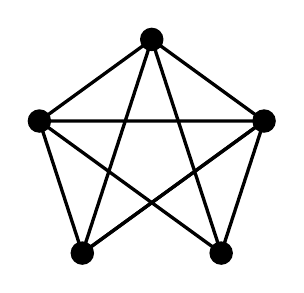
\begin{tikzpicture}
        \draw[very thick]  (18:1.5) \foreach \a in {90,162,234} { --
        (\a:1.5) } -- cycle;
        \draw[very thick] (18:1.5) \foreach \a in {162,306,90,234} {
        -- (\a:1.5) } -- cycle;
        \draw[very thick] (18:1.5) \foreach \a in {306,18} { -- (\a:1.5) };
        \foreach \a in {18,90,162,234,306} {
        \node[black,fill=black,circle,inner sep=3pt] at (\a:1.5){}; }
      \end{tikzpicture}
    }
    \uncover<4->{\caption{The complete multipartite graph
      \emph{$K_{1,1,1,2}$} on 5 vertices.}
    \label{fig:quantum-network-example}}
  \end{figure}
}

\frame{
  \frametitle{Quantum Computers/Networks}
  \begin{defn}[Perfect State Transfer]A quantum network with
    localities $u \perp v$ exhibits \emph{perfect state transfer}
    over a period $T$ of unitary evolution if and only if a qubit
    $p$'s \emph{wave function} satisfies $\vert\Psi(p \in u,
    t_0)\vert = \vert\Psi(p \in v, t_0 + T)\vert = 1$.
  \end{defn}\medskip

  \begin{itemize}
      \uncover<2->{
      \item \emph{i.e.,} when a particle holding quantum information
        completely ``redistributes'' from node $u$ at time $t_0$ to
      node $v$ at time $t_0 + T$}
      \uncover<3->{
      \item Perfect state transfer (PST) thus facilitates
        \emph{high-fidelity} information transmission in quantum
      communication systems}
      \uncover<4->{
      \item A qubit's position is a probability distribution (``wave
        function'') rather than a precise location, so PST is not easy
      to achieve\ldots}
      \uncover<5->{
      \item \ldots but a certain property of network graph
        representations called \emph{$S$-bandwidth} serves as an
      indicator in some cases}
  \end{itemize}
}

%%%%%%%%%%%%%%%%%%%%%%%%%%%%%%%%%%%%%%%%
\subsection{\textit{S}-Bandwidth and PST}
%%%%%%%%%%%%%%%%%%%%%%%%%%%%%%%%%%%%%%%%

\frame{
  \frametitle{$S$-Bandwidth and PST}

  A small number of \emph{Laplacian integral} graphs are
  \emph{$\{-1,1\}$-} and \emph{$\{-1,0,1\}$-diagonalizable}. This can
  be an indicator of PST in quantum networks.\medskip
  \uncover<2->{
    \begin{defn}[Matrix Bandwidth]A matrix $X$ has a \emph{matrix
      bandwidth} of $\beta(X) = k$ if and only if $x_{ij} = 0$
      whenever $\vert i - j \vert \geq k$.
  \end{defn}\medskip}
  \begin{itemize}
      \uncover<3->{
    \item For instance, the following matrix has a bandwidth of $2$:}
  \end{itemize}
  \uncover<3->{
    \begin{align*}
      \begin{bmatrix}
        1 & 2 & 0 & 0 & 0 & 0 \\
        4 & 0 & 5 & 0 & 0 & 0 \\
        0 & 4 & 6 & 1 & 0 & 0 \\
        0 & 0 & 0 & 4 & 3 & 0 \\
        0 & 0 & 0 & 3 & 3 & 7 \\
        0 & 0 & 0 & 0 & 5 & 0
      \end{bmatrix}
  \end{align*}}
}

\frame{
  \frametitle{$S$-Bandwidth and PST}
  \begin{defn}[Graph $S$-Bandwidth]A graph $G$ has an
    \emph{$S$-bandwidth} of $\beta_S(G) = k$ if and only if $L(G) =
    PDP^{-1}$ for some $P \in S^{n \times n} \subseteq \mathbb{R}^{n
    \times n}$ with $\beta(P^TP) = k$.
  \end{defn}\medskip

  \begin{itemize}
      \uncover<2->{
      \item \emph{i.e.,} when $G$'s \emph{Laplacian matrix} has a full
        set of eigenvectors $\mathbf{v}_1, \mathbf{v}_2, \ldots,
        \mathbf{v}_n \in S^{n}$ such that $\mathbf{v}_i \cdot
      \mathbf{v}_j = 0$ whenever $\vert i - j \vert \geq k$}
      \uncover<3->{
      \item We say that a graph is \emph{$S$-diagonalizable} if its
        $S$-bandwidth is finite\textemdash when $S = \{-1,1\}$ or
      $\{-1,0,1\}$, this may indicate PST}
      \uncover<4->{
      \item To test a graph for $\{-1,1\}$- and
        $\{-1,0,1\}$-diagonalizability and determine its exact
        bandwidths, we first need to find the eigenvectors of its
      Laplacian matrix\ldots}
  \end{itemize}
}

%%%%%%%%%%%%%%%%%%%%%%%%%%%%%%%%%%%%%%%%
\section{Algorithm Breakdown and Analysis}
%%%%%%%%%%%%%%%%%%%%%%%%%%%%%%%%%%%%%%%%

%%%%%%%%%%%%%%%%%%%%%%%%%%%%%%%%%%%%%%%%
\subsection{Identifying \{-1,0,1\}-Eigenvectors}
%%%%%%%%%%%%%%%%%%%%%%%%%%%%%%%%%%%%%%%%

\frame{
  \frametitle{Identifying $\{-1,0,1\}$-Eigenvectors}

  \begin{itemize}
    \item The \emph{linear conditions} we have identified give the
      following bound on $\{-1,0,1\}$-eigenvectors for an order $n$ Laplacian:
  \end{itemize}
  \begin{align*}
    \frac{1}{2}\sum_{k = 1}^n\binom{n}{k}\binom{n - k}{k} \leq 3^{n -
    2} \ \ \forall n \in \mathbb{N}
  \end{align*}

  \begin{itemize}
      \uncover<2->{
      \item Therefore, eigenvector identification has \emph{complexity
      $O(3^{n - 2})$}}
      \uncover<3->{
      \item This \emph{exponential increase} in the number of
        eigenvectors to check is one of our two main bottlenecks\ldots
      unfortunately, this seems to already be the theoretical lower bound}
  \end{itemize}
}

%%%%%%%%%%%%%%%%%%%%%%%%%%%%%%%%%%%%%%%%
\subsection{Finding \textit{k}-Orthogonal Bases}
%%%%%%%%%%%%%%%%%%%%%%%%%%%%%%%%%%%%%%%%

\frame{
  \frametitle{Finding $k$-Orthogonal Bases}

  Now, we have all $\{-1,0,1\}$-eigenvectors \emph{stored as columns
  in matrices} (one for each eigenspace):\medskip
  \begin{align*}
    \textbf{Eigenspace 1:} \quad \bigl[
      \mathbf{v}_{\lambda_1, 1} \mid \mathbf{v}_{\lambda_1, 2} \mid &
      \ldots \mid \mathbf{v}_{\lambda_1, r_1}
    \bigr]\\
    \textbf{Eigenspace 2:} \quad \bigl[
      \mathbf{v}_{\lambda_2, 1} \mid \mathbf{v}_{\lambda_2, 2} \mid &
      \ldots \mid \mathbf{v}_{\lambda_2, r_2}
    \bigr]\\
    & \:\:\, \vdots \\
    \textbf{Eigenspace } \bm{k}\textbf{:} \quad \bigl[
      \mathbf{v}_{\lambda_k, 1} \mid \mathbf{v}_{\lambda_k, 2} \mid &
      \ldots \mid \mathbf{v}_{\lambda_k, r_k}
    \bigr]
  \end{align*}

  \begin{itemize}
      \uncover<2->{
      \item If any eigenspace contains less $\{-1,0,1\}$-eigenvectors
      than its multiplicity, the graph is not $\{-1,0,1\}$-diagonalizable}
      \uncover<3->{
      \item Otherwise, convert each matrix to RREF (saving the pivots)
      to verify that we have enough \emph{linearly independent} eigenvectors}
      \uncover<4->{
    \item Similarly, test for $\{-1,1\}$-diagonalizability}
  \end{itemize}
}

\frame{
  \frametitle{Finding $k$-Orthogonal Bases}

  We must find not only linearly independent eigenbases, but those
  with minimum \emph{$k$-orthogonality} (i.e., with a Gram matrix
  $P^TP$ of bandwidth $k$). Since matrix bandwidth is
  \emph{permutation-variant}:

  \begin{itemize}
      \uncover<2->{
      \item For \emph{$k = 1$} (pairwise orthogonality): Check whether
      the Gram matrix of the basis set is \emph{diagonal}}
      \uncover<3->{
      \item For \emph{$k = 2$} (quasi-orthogonality): Check whether the
        Gram matrix of the basis is the adjacency matrix of a
      \emph{path subgraph}}
      \uncover<4->{
      \item For \emph{$2 < k < n$}: Here we must resort to some more
        complex \emph{subgraph isomorphism} tests, which can still be
      improved\ldots}
  \end{itemize}
}

\frame{
  \frametitle{Finding $k$-Orthogonal Bases}

  Now to actually find a basis\ldots

  \begin{itemize}
      \uncover<2->{
      \item We construct a search tree of \emph{eigenvector indices},
      starting from roots with one index each}
      \uncover<3->{
      \item Create children by adding column indices corresponding to
        eigenvectors, only keeping options that preserve linear
      independence and maintain $k$-orthogonality}
      \uncover<4->{
      \item Conduct a \emph{depth-first search} on this \emph{lazily
      constructed tree} until a $k$-orthogonal basis is found}
      \uncover<5->{
    \item If no basis is found, repeat for $(k + 1)$-orthogonality \ldots}
      \uncover<6->{
    \item Perform a search for $\{-1,1\}$-bandwidth as well if appropriate}
      \uncover<7->{
      \item Unfortunately, this search tree grows in \emph{factorial
      time}, making it another bottleneck\ldots}
  \end{itemize}
}

%%%%%%%%%%%%%%%%%%%%%%%%%%%%%%%%%%%%%%%%
\subsection{Minimizing \textit{S}-Bandwidth}
%%%%%%%%%%%%%%%%%%%%%%%%%%%%%%%%%%%%%%%%

\frame{
  \frametitle{Minimizing $S$-Bandwidth}

  We can now use these foundations to construct the first algorithm
  to compute a graph's $S$-bandwidth!
  \begin{itemize}
    \item First, we check each eigenspace for a \emph{$k$-orthogonal
      basis} up to $k = \mu - 1$ (where $\mu$ is the dimension of the
      eigenspace)
      \uncover<2->{
      \item If no $(\mu - 1)$-orthogonal basis is found, we use the
      pivots from our original row reduction to get a $\mu$-orthogonal basis}
      \uncover<3->{
      \item With every test, save the value of $k$ and only start
        checking subsequent eigenspaces against that
      \emph{orthogonality parameter}}
      \uncover<4->{
      \item Complete this process for all eigenspaces to minimize the
      overall $S$-bandwidth of the graph, and we are done!}
  \end{itemize}
}

%%%%%%%%%%%%%%%%%%%%%%%%%%%%%%%%%%%%%%%%
\section{Results, Findings, and Future Work}
%%%%%%%%%%%%%%%%%%%%%%%%%%%%%%%%%%%%%%%%

%%%%%%%%%%%%%%%%%%%%%%%%%%%%%%%%%%%%%%%%
\subsection{Results / Findings / Future Work}
%%%%%%%%%%%%%%%%%%%%%%%%%%%%%%%%%%%%%%%%
\frame{
  \frametitle{Results / Findings / Future Work}

  We have tabulated, with exact $\{-1,1\}$- and $\{-1,0,1\}$-bandwidths,\medskip
  \begin{itemize}
      \uncover<2->{
      \item all $\{-1,0,1\}$-diagonalizable \emph{simple connected
      graphs} on $n \leq 11$ vertices, and}
      \uncover<3->{
      \item all $\{-1,0,1\}$-diagonalizable \emph{simple connected
        regular graphs} (a superset of the \emph{bipartite} ones) on $n
      \leq 14$ vertices}
  \end{itemize}

  \uncover<4->{We have also proven several results about the
    \emph{Laplacian spectra} of $S$-diagonalizable graphs, the effects
    of different \emph{edge weights} on $S$-bandwidths, and
  $S$-diagonalizable \emph{graph composition}.\medskip}

  \uncover<5->{Next, we hope to improve methods of \emph{matrix
    bandwidth reduction}, reduce the complexity of our \emph{DFS search
  tree}, investigate remaining conjectures on $S$-diagonalizable graphs.}
}

\frame{
  \frametitle{Results / Findings / Future Work}
  \begin{figure}
    \centering
    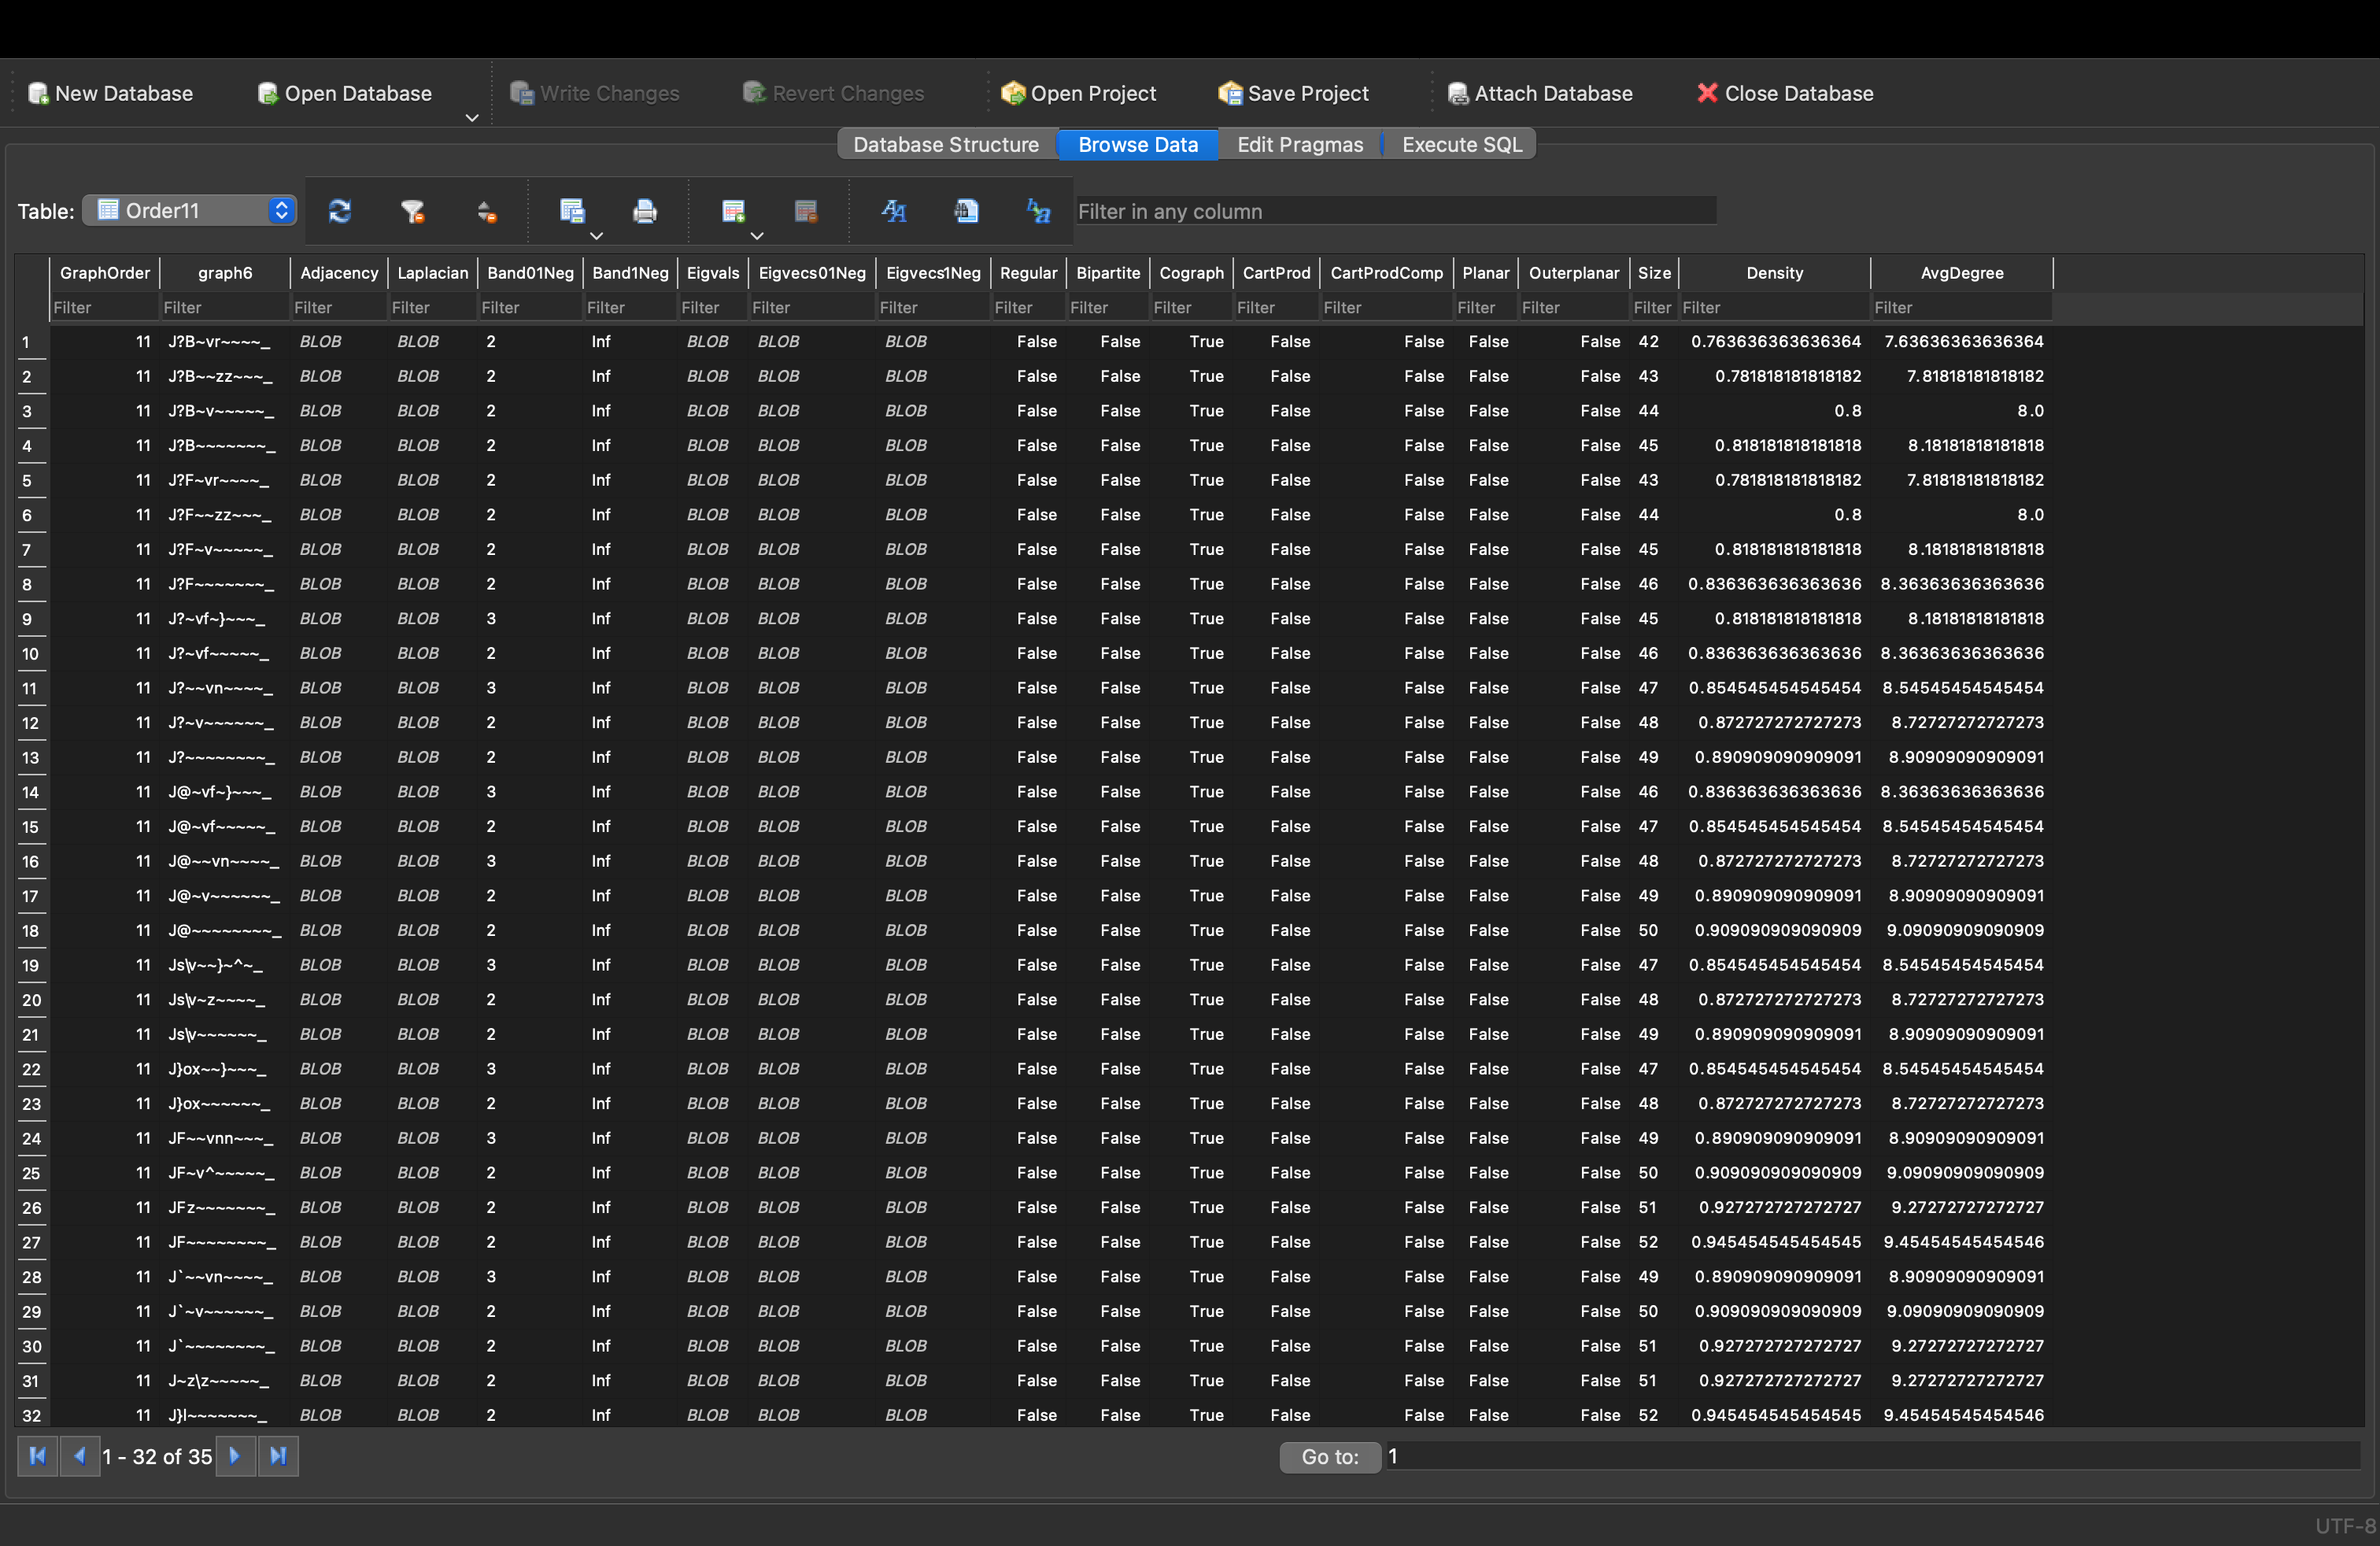
\includegraphics[height=6.6cm]{assets/tabular_data.png}
    \caption{Some tabulated data on $\{-1,0,1\}$-diagonalizable graphs.}
    \label{fig:tabular-data}
  \end{figure}
}

%%%%%%%%%%%%%%%%%%%%%%%%%%%%%%%%%%%%%%%%
\subsection{Thank you!}
%%%%%%%%%%%%%%%%%%%%%%%%%%%%%%%%%%%%%%%%

\frame{
  \frametitle{Thank you!}
  \begin{figure}
    \centering
    
\includegraphics[height=6.6cm]{assets/pusheen_thank_you.png}
    \caption{Pusheen the Cat \textless 3}
    \label{fig:pusheen-thank-you}
  \end{figure}
}

\end{document}
